\documentclass{article}
\usepackage[utf8]{inputenc}

\title{Using overleaf for writing and integrating with Jupyter and Github}
\author{Arindam Basu}
\date{October 2018}

\usepackage{natbib}
\usepackage{graphicx}

\begin{document}

\maketitle

\section{Introduction}
Overleaf is an excellent tool and works well for productive work. In this tutorial, I am going to use a low end machine running Arch Linux with pandoc and jupyter notebook and git installed. My goal will be to first create an article (this one) in Overleaf, with initial ideas of plans and data analyses, and then I will use github and git to work with the article by adding analyses to produce an article that will then get pushed to online repositories for publishing. This will demonstrate that a workflow is possible using only plain text integrating latex and markdown and other tools that are not resource heavy but can be used gainfully without the need for using resource intensive and non-free or non-open source tools for data analysis and writing fairly complex texts. 

For this to work, we will use the following tools and processes:

\begin{itemize}
    \item Overleaf as a starter document
    \item Push the document in Overleaf to github
    \item Set up a git repo or clone the git repo on the local machine
    \item In the same directory, open a new jupyter notebook
    \item read data, conduct data analyses
    \item write the document in the jupyter notebook using markdown
    \item convert the notebook *.ipynb file to latex
    \item connect to the github repo using git
    \item read it back in overleaf and change or edit as the final piece

\end{itemize}

With a workflow such as this, it is important to keep some processes separate. First, while overleaf can be a starter and finisher of the document, some processes need to be carefully reviewed such that a latex document created here does not necessarily play well in the jupyter notebook unless using git and pandoc one can faithfully translate the documents, so a caution might be useful. Also, while in jupyter using markdown, it is easy to insert citations, they are best avoided using the markdown syntax of [@citation\_id].



\begin{figure}[h!]
\centering
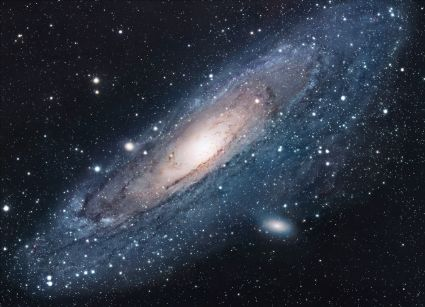
\includegraphics[scale=1.7]{universe}
\caption{The Universe}
\label{fig:universe}
\end{figure}

\section{Conclusion}
``I always thought something was fundamentally wrong with the universe'' \citep{adams1995hitchhiker}

\bibliographystyle{plain}
\bibliography{references}
\end{document}
